\subsection{Top Down Model}

A second method for creating absolute arguments is proposed here that considers the assertion as a whole. Where the previous model constructed the assertion from an empty set, the Top Down approach goes through a similar process in reverse. Consider \cref{fig:hesse} as a form of search tree to serve as an example. Beginning at $W = \{S_1, S_2, S_3 \}$, this scheme iteratively removes states from consideration, descending the tree, until the probability of the assertion is below a certain threshold $\gamma$. This prevents the speaker from asserting an argument that it did not have enough probability in as a whole. This can be written as 

\begin{equation} \label{eq:TD_approach}
    \mathbf{A} = \{ S_i: p(\mathbf{S}) \leq \gamma  \}
\end{equation}


It is clear that this method aims to propose the most specific assertion it can, removing states for which $p_i$ is low however it scales badly at $O(2^n)$. It should be noted that, for both models, $\gamma$ is imposed to prevent the speaker making statements for which is has low probability. However, in the top down approach the significance applies to the argument as a whole and so is a much less prescriptive condition. 


\begin{figure}[H]
    \centering
    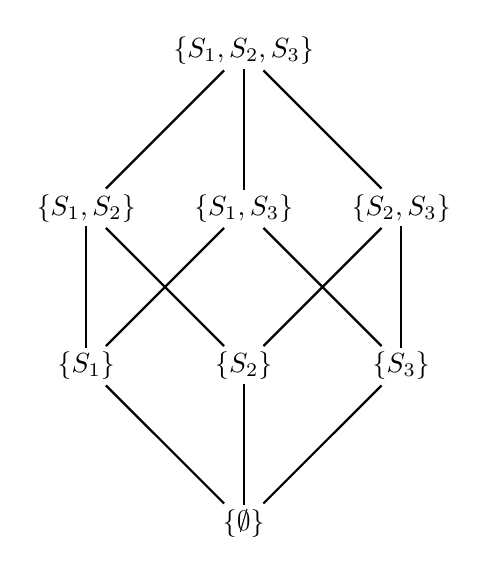
\begin{tikzpicture}
    % First, locate each of the nodes and name them
        \node (top) at (0,0) {$\{S_1, S_2, S_3\}$};
        \node (left) at (-2, -2) {$\{S_1, S_2\}$};
        \node (center) at (0, -2) {$\{S_1, S_3\}$};
        \node (right) at (2, -2) {$\{S_2, S_3\}$};
        \node (one) at (-2, -4) {$\{S_1\}$};
        \node (two) at (0, -4) {$\{S_2\}$};
        \node (three) at (2, -4) {$\{S_3\}$};
        \node (empty) at (0, -6) {$\{\emptyset \}$};

    % Now draw the lines:
        \draw [thick, shorten <=-2pt, shorten >=-2pt] (top) -- (left);
        \draw [thick, shorten <=-2pt, shorten >=-2pt] (top) -- (center);
        \draw [thick, shorten <=-2pt, shorten >=-2pt] (top) -- (right);
        \draw [thick, shorten <=-2pt, shorten >=-2pt] (left) -- (one);
        \draw [thick, shorten <=-2pt, shorten >=-2pt] (left) -- (two);
        \draw [thick, shorten <=-2pt, shorten >=-2pt] (center) -- (one);
        \draw [thick, shorten <=-2pt, shorten >=-2pt] (center) -- (three);
        \draw [thick, shorten <=-2pt, shorten >=-2pt] (right) -- (two);
        \draw [thick, shorten <=-2pt, shorten >=-2pt] (right) -- (three);
        \draw [thick, shorten <=-2pt, shorten >=-2pt] (one) -- (empty);
        \draw [thick, shorten <=-2pt, shorten >=-2pt] (two) -- (empty);
        \draw [thick, shorten <=-2pt, shorten >=-2pt] (three) -- (empty);
    \end{tikzpicture}   
    \caption{A Hesse Diagram for a world with 3 possible states}
    \label{fig:hesse}
\end{figure}
